\section{Error Handling}\label{error-handling-chap}
We won't be discussing another visitor in the section, we will however be describing how the Ezuino compiler handles errors in general.\\
Error Handling is a vital general tool, which is used for the users to get an overview of the errors, which they made during their time coding the Ezuino programming language. The Ezuino error handling tool also implements a small part of the ANTLR Runtime library, which detects errors in the syntax.
\\\\
The Ezuino error handling system can be described in two parts. The first part is the part implementing the ANTLR Runtime libary. The second part is Ezuino's own custom error handling system.
\\\\
Ezuino uses the ANTLR libary to implement it's own version of the \texttt{ANTLRErrorListener} class. This is implemented in the class named: \texttt{ErrorListener}. The \texttt{ErrorListener} is used to check the data ANTLR generates, for syntax errors. If no syntax errors is found in the ANTLR generated data, the compiler continues.\\
However, if an error is found, it is added to a list of errors held within the \texttt{ErrorHandler} class. The \texttt{ErrorHandler} class is part of Ezuino's custom error system and will be described later.\\
Listing \ref{eh01} shows the implementation of the \texttt{ErrorListener} class and how it uses the \texttt{ErrorHandler} class to add a \texttt{syntaxError} to the handler class.\\
\begin{lstlisting}[caption={Start of the ErrorListener class}, label={eh01}]
private int errorCount;
private ErrorHandler errorHandler;

public ErrorListener(ErrorHandler errorHandler) {
    this.errorHandler = errorHandler;
    this.errorCount = 0;
}

$$@Override
public void syntaxError(Recognizer<?, ?> recognizer, Object offendingSymbol, int line, int charPositionInLine,
    String msg, RecognitionException e) {
    this.errorCount++;
    errorHandler.syntaxError(errorCount, msg, line, charPositionInLine);
}
\end{lstlisting}
\noindent\newline
Next we have Ezuino's own custom error handling system. As mentioned, the \texttt{ErrorHandler} class in part of this system. The \texttt{ErrorHandler} class also functions as the main class of Ezuino's error system. It's the class responsible for handling all errors that occurs in the compiler. The \texttt{ErrorHandler} (handler) holds a list of errors and a \texttt{errorCount} which it uses to keep track of all errors given to it. During compiling, Ezuino regularly checks that the handler has no errors. These checks occurs after each section, a section being either the syntax or contextual analysis. If one or more errors has occurs during one of the sections, the compiler will stop after the section and print the errors to the user.\\
Listing \ref{eh03} shows a code snippet of the \texttt{ErrorHandler}. On it, is the error message, error count and public method for printing all of the errors in the list.\\
\begin{lstlisting}[caption={Start of ErrorHandler class}, label={eh03}]
private List<ErrorMessage> messageList = new ArrayList<>();
private int errorCount = 0;

public boolean hasErrors() {
    return errorCount != 0;
}

public void printErrors(String reason) {
    if (hasErrors()) {
        StringBuilder sb = new StringBuilder();
        String errmsg = "##  " + reason + "\n -- ## ERROR OUTPUT CONSOLE ## -- ";
        sb.append(errmsg + "\n");
        for (ErrorMessage message : messageList) {
            sb.append(message + "\n");
        }
        System.err.println(sb.toString());
    }
}
\end{lstlisting}
\noindent\newline
Just like the \texttt{ErrorListener} used the handler class to add errors, the visitors of Ezuino can also use the handler class to add errors that might occur during their execution. Because the visitors can use handler class to report their errors, it's possible to divide the compiler into different sections, as described earlier.
\\\\



Listing \ref{eh04} shows three examples of different errors the visitors can use to give detailed error messages to the user.
\begin{lstlisting}[caption={three different error messages from the ErrorHandler class}, label={eh04}]
public void syntaxError(int errorCount, String msg, int line, int charPositionInLine) {
    String errorMsg = String.format("#" + errorCount + " - " + "Error parsing expression: '%s' on line %s, position %s", msg, line, charPositionInLine);
    addError(new SyntaxError(ErrorType.ERROR, errorMsg));
}
public void funcAlreadyDeclared(String character) {
    addError(new GeneralError(ErrorType.ERROR, "Function " + character + " is already defined in this scope."));
}
public void unexpectedType(ITypeNode node, Type type) {
    addError(new GeneralError(ErrorType.ERROR, "Unexpeced type! Expected: " + type.name() + ", was " + node.getType().name() + " - Node: " + node));
}
\end{lstlisting}
\noindent\newline




The \texttt{ErrorListener} class implements the \texttt{ANTLRErrorListener} interface, which is used for implementing methods for the different kinds of ANTLR errors. This allows the listener to syntax errors.

The one we’re interested in is shown in listing \ref{eh01}. In this code, we’re inside the \texttt{ErrorListener} class, which implements the \texttt{ANTLRErrorListener} interface. In listing \ref{eh01}, one global variables exist. The global variable: \texttt{errorCount}, which is used to count the number of errors, ANTLR found during the parsing.\\
The ErrorHandler instantiation is from the ErrorHandler class, which handles a specific type of errors during the AST and covers more abstract error handling, for example, cast exceptions, type exceptions and many more. The \texttt{ErrorHandler} class will be described later in this section.
\\\\
The only method we are interested in is the \texttt{syntaxError} method, which is recognizing syntax errors made by the users. As an example, if the users input the code (int int), this would be a violation of the ANTLR grammar, as it’s two literals, the scanner review as int type declarations, without any ID after both the declarations. If the scanner recognizes this error, it will not run the visitors, or future visitors through, as the error was caught in the earlier stages of the process.
\\\\
Going back to the ErrorHandler class, we got 3 methods, which has the main functionality of the error handler. 
\begin{lstlisting}[caption={Start of ErrorHandler class}, label={eh03}]
private List<ErrorMessage> messageList = new ArrayList<>();
private int errorCount = 0;

public boolean hasErrors() {
    return errorCount != 0;
}

public void printErrors(String reason) {
    if (hasErrors()) {
        StringBuilder sb = new StringBuilder();
        String errmsg = "##  " + reason + "\n -- ## ERROR OUTPUT CONSOLE ## -- ";
        sb.append(errmsg + "\n");
        for (ErrorMessage message : messageList) {
            sb.append(message + "\n");
        }
        System.err.println(sb.toString());
    }
}
\end{lstlisting}
\noindent\newline
Listing \ref{eh03}, is a snippet from the ErrorHandler class. On line 1, we got a List, which contains all the error messages found during the contextual analysis, reported by errors in the AST visitor classes. The method hasErrors() from line 4, checks if the errorCount on line 2, is bigger than 0. If it is, that means that the error handler has added an error to the error list.\\
Finally, from line 13 we got the printErrors() method, which prints the methods, which is in listing \ref{eh04}. First, it checks whenever there are errors, then it prints all the messages in the List, by running a for each loop for 18. 
\begin{lstlisting}[caption={three different error messages from the ErrorHandler class}, label={eh04}]
public void syntaxError(int errorCount, String msg, int line, int charPositionInLine) {
    String errorMsg = String.format("#" + errorCount + " - " + "Error parsing expression: '%s' on line %s, position %s", msg, line, charPositionInLine);
    addError(new SyntaxError(ErrorType.ERROR, errorMsg));
}
public void funcAlreadyDeclared(String character) {
    addError(new GeneralError(ErrorType.ERROR, "Function " + character + " is already defined in this scope."));
}
public void unexpectedType(ITypeNode node, Type type) {
    addError(new GeneralError(ErrorType.ERROR, "Unexpeced type! Expected: " + type.name() + ", was " + node.getType().name() + " - Node: " + node));
}
\end{lstlisting}
\noindent\newline
Listing \ref{eh04} has 3 methods, which is being used within the visitors. The methods take either string as ID’s, or nodes and do in-method conversions of messages, which are being added to the List on listing \ref{eh03}, line 1. The SyntaxError and GeneralError classes both contain different string representations of each error. 
\begin{lstlisting}[caption={The syntaxError class}, label={eh05}]
public class SyntaxError extends ErrorMessage{

    public SyntaxError(ErrorType errorType , String errorMessage) {
        super(errorType, errorMessage);
    }

    $$@Override
    public String toString() {
        return String.format("SYNTAX %s %s", this.getTypeString().toUpperCase(), this.getErrorDescription());
    }
}
\end{lstlisting}
\noindent\newline
Listing \ref{eh05} is an example of the SyntaxError class, for every error method in Listing \ref{eh04}, which constructs a new SyntaxError, will need the input of an Error Type and Error Message. Then, the toString() method from line 8, returns a string with a specific format, for this syntax error. 
To get an overview of these classes together, a relationship diagram has been created and can be reviewed in figure \ref{eh06} below.
\begin{figure}[H]
\centering
\frame{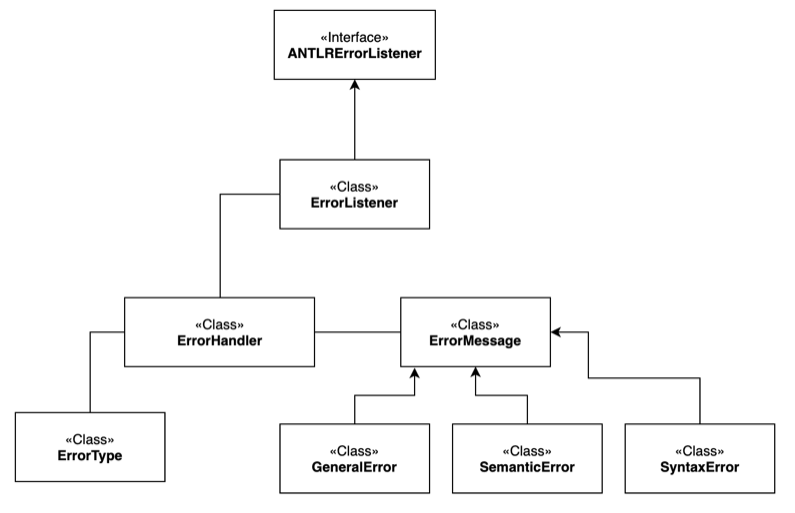
\includegraphics[scale=0.45]{figures/implementation/errorHandler/eh06.png}}
\caption{Diagram of the error classes}
\label{eh06}
\end{figure}
Figure \ref{eh06} uses the ANTLRErrorListener interface to overwrite with a new class named ErrorListener, which is then associated with the ErrorHandler. The ErrorHandler got a ErrorType and ErrorMessage, which there are three versions (GeneralError, SemanticError and SyntaxError).\\
As we are done going through the different visitors and its implementation, we can now move on towards testing the compiler.